\documentclass[12pt]{article}
\usepackage[UTF8]{ctex}
\usepackage{geometry}
\usepackage{listings}
\usepackage{graphicx}
\usepackage{subfigure}
\usepackage{array}
\usepackage{caption}    
\usepackage{float}
\usepackage{subfloat}
\usepackage{hyperref}
\usepackage{bookmark}
\usepackage{amsmath}
\usepackage{url}
\usepackage{amsfonts,amssymb}

\geometry{left=15mm,right=15mm,top=20mm,bottom=20mm}
\title{第八次作业报告}
\author{PB21010362 汪兆辰}
\date{\today}
\newcommand{\upcite}[1]{\textsuperscript{\textsuperscript{\cite{#1}}}}

\begin{document}

\maketitle

\section{算法介绍}

由于参数化前后的三角网格具有一一对应关系,只需对参数化后的二维网格进行贴图就可以得到经纹理映射的三维网格. 但由于二维网格的采样是离散的,容易出现锯齿,可以利用GL中的一些纹理
过滤方法,例如对附近像素进行插值的线性过滤,使得图案更平滑.

为了实现在三角网格上的纹理贴图,需要将给定的网格参数化,这里用到HW5的tutte参数化内容. 由于给定的纹理为512*512的正方形图像,为了方便贴图,将HW5稍作修改,使其
将给定网格参数化映射到正方形中,结果如下,
\begin{figure}[htbp]
    \centering
    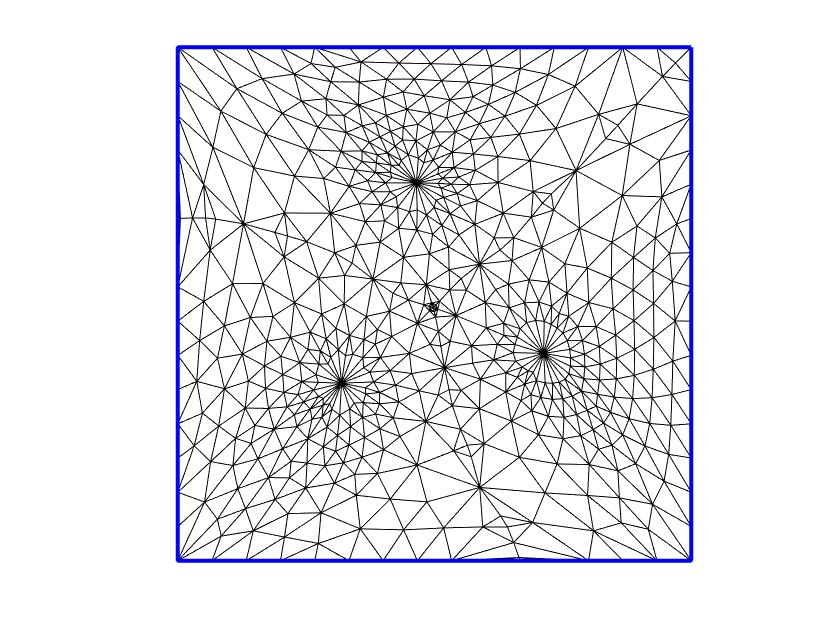
\includegraphics[scale=0.5]{pic01.jpg}
\end{figure}
并将得到的参数坐标以csv文件格式输出.

为了方便,本次作业在HW6的框架上进行修改. 在主函数中读入csv文件并将其存储在vector中. 注意到读取文件过程中数据以字符串格式存储,需要用到atof函数将字符串转换为float类型. 
得到参数点的坐标后,将其数据上传到网格对象,设置贴图为给定的纹理,并设置边界处理方式等,再将对象的showTexture属性改为true即可显示纹理.

\section{实现效果}
\begin{figure}[htbp]
    \centering
    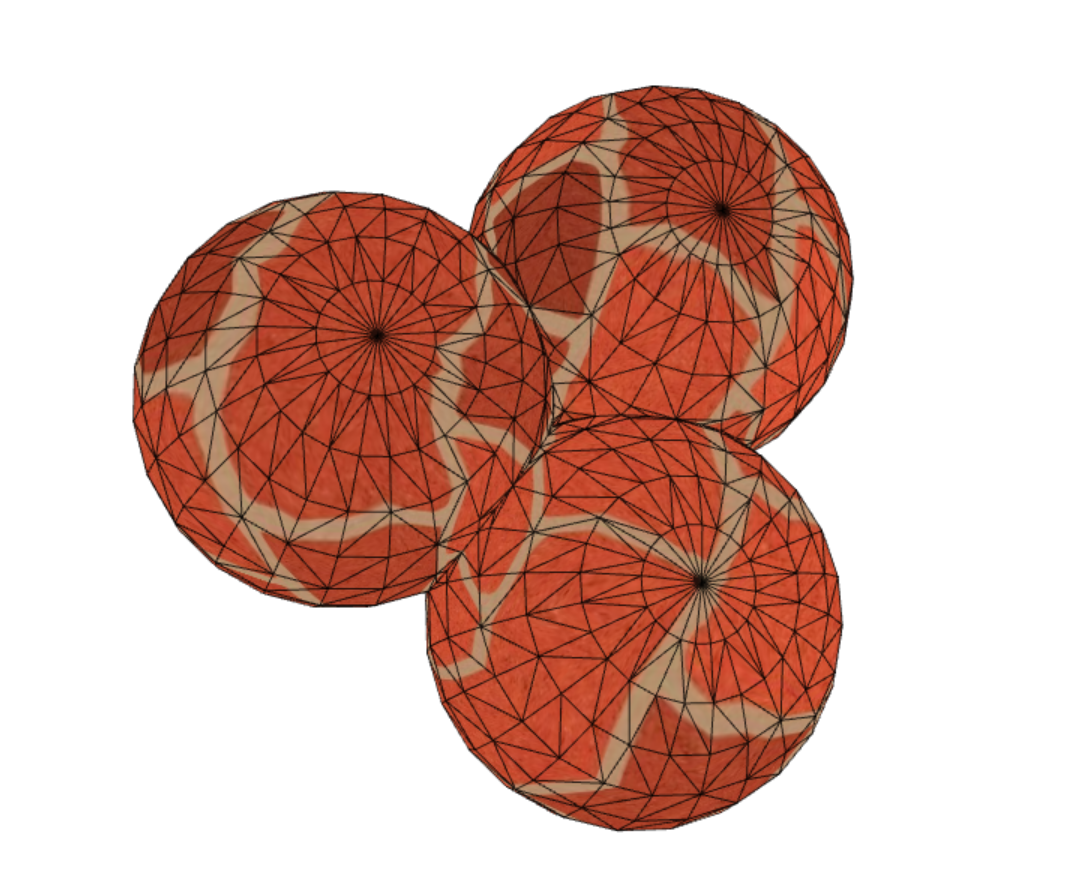
\includegraphics[scale=0.5]{pic02.png}
\end{figure}


\begin{thebibliography}{3}
    \bibitem{1} \url{https://learnopengl-cn.github.io/01%20Getting%20started/06%20Textures/}
    \bibitem{2} \url{https://zhuanlan.zhihu.com/p/369977849}
\end{thebibliography}

\end{document}